\documentclass[tikz,border=12pt]{standalone}
\usepackage[T1]{fontenc}
\usepackage{mathpazo}
\usepackage{amsmath,amssymb}
\usetikzlibrary{arrows.meta, positioning, calc, fit, decorations.pathreplacing}

\definecolor{stblue}{HTML}{7B97AD}
\definecolor{rwgold}{HTML}{B8995E}
\definecolor{sage}{HTML}{7A9A7E}
\definecolor{dkbrown}{HTML}{3D3530}
\definecolor{wmgray}{HTML}{7B7067}
\definecolor{cream}{HTML}{F9F6F0}
\definecolor{border}{HTML}{D4C9B8}
\definecolor{terracotta}{HTML}{C47A6A}

\begin{document}
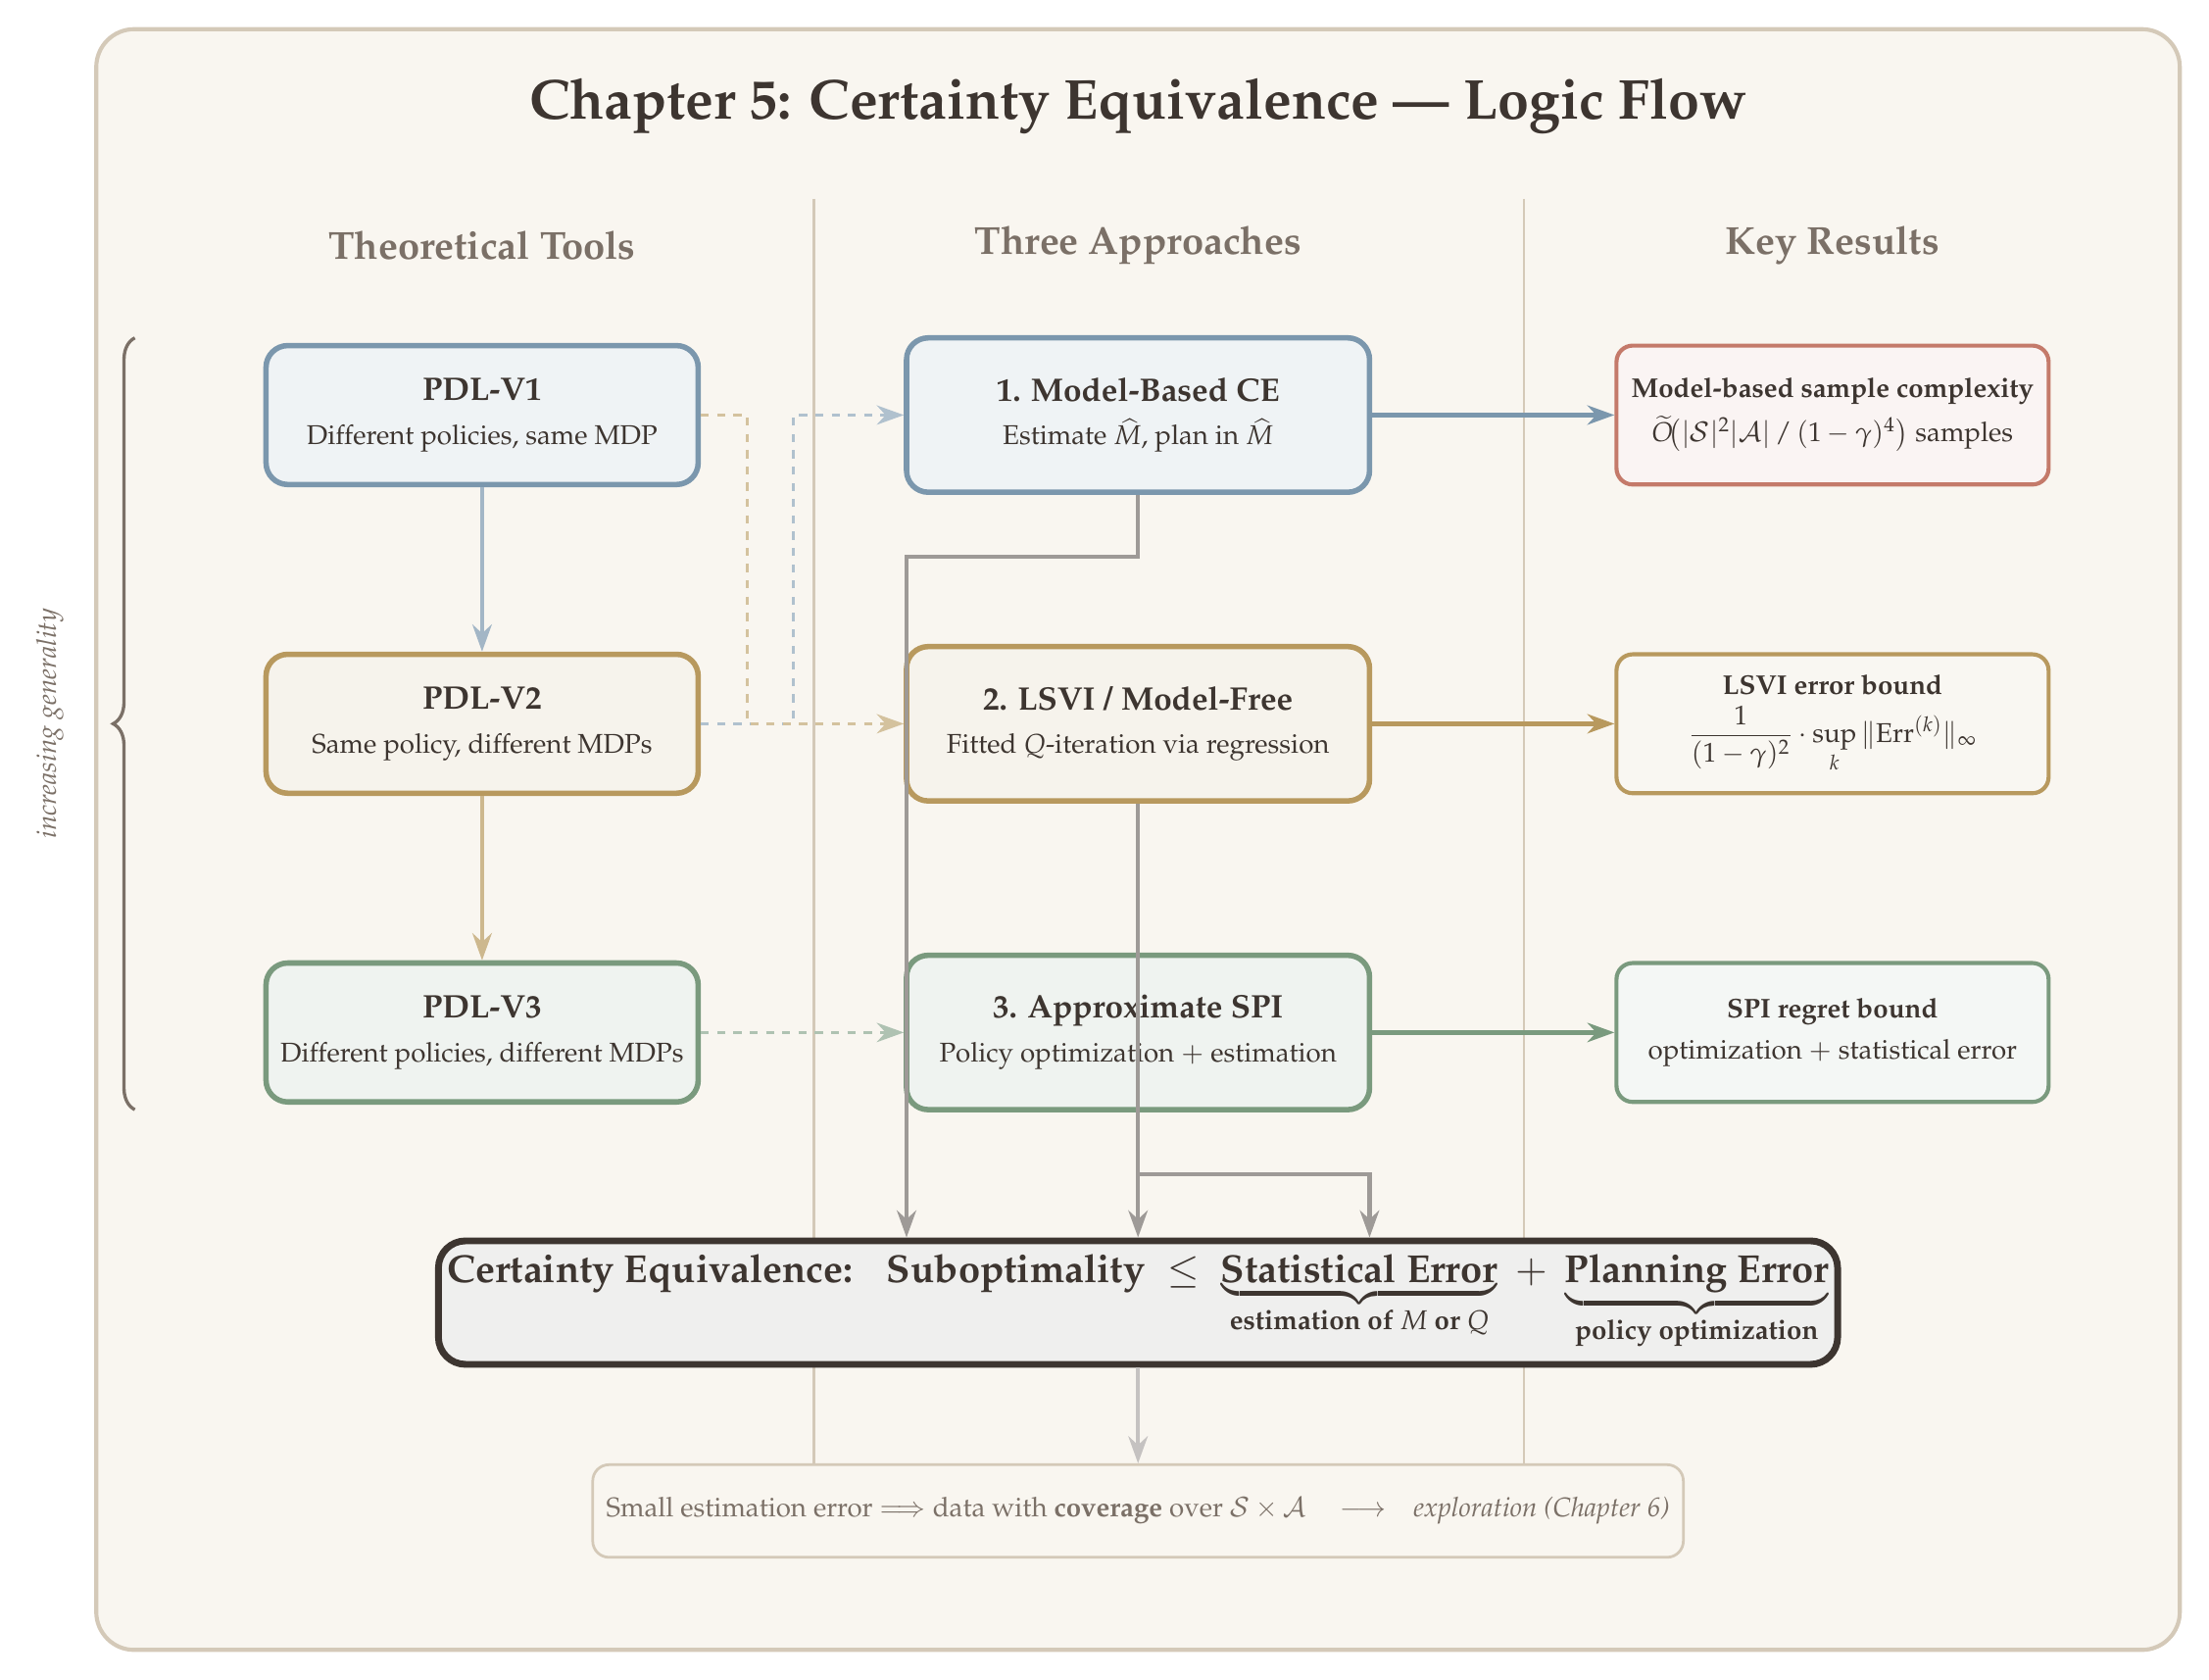
\begin{tikzpicture}[
  >={Stealth[length=3.5mm, width=2.5mm]},
  toolbox/.style={draw=#1, line width=2pt, fill=#1!12, rounded corners=8pt,
    minimum width=56mm, minimum height=18mm, font=\large\bfseries, text=dkbrown,
    align=center, inner sep=5pt},
  approach/.style={draw=#1, line width=2pt, fill=#1!12, rounded corners=8pt,
    minimum width=60mm, minimum height=20mm, font=\large\bfseries, text=dkbrown,
    align=center, inner sep=5pt},
  result/.style={draw=#1, line width=1.5pt, fill=#1!8, rounded corners=6pt,
    minimum width=56mm, minimum height=18mm, font=\normalsize, text=dkbrown,
    align=center, inner sep=5pt},
  arr/.style={->, line width=1.6pt, dkbrown},
  darr/.style={->, line width=1.2pt, dashed, wmgray},
]

% Background
\fill[cream, rounded corners=14pt] (-1.5,-16.0) rectangle (25.5,5.0);
\draw[border, rounded corners=14pt, line width=1.5pt] (-1.5,-16.0) rectangle (25.5,5.0);

% Title
\node[font=\huge\bfseries, text=dkbrown] at (12.0,4.0)
  {Chapter 5: Certainty Equivalence --- Logic Flow};

% =============================================
% Column headers
% =============================================
\node[font=\Large\bfseries, text=wmgray] at (3.5,2.2) {Theoretical Tools};
\node[font=\Large\bfseries, text=wmgray] at (12.0,2.2) {Three Approaches};
\node[font=\Large\bfseries, text=wmgray] at (21.0,2.2) {Key Results};

% Thin vertical separators
\draw[border, line width=1pt] (7.8,2.8) -- (7.8,-14.8);
\draw[border, line width=1pt] (17.0,2.8) -- (17.0,-14.8);

% =============================================
% Left column: Theoretical Tools (PDL versions)
% =============================================
\node[toolbox=stblue] (pdl1) at (3.5,0.0)
  {PDL-V1\\[2pt]\normalfont\normalsize Different policies, same MDP};

\node[toolbox=rwgold] (pdl2) at (3.5,-4.0)
  {PDL-V2\\[2pt]\normalfont\normalsize Same policy, different MDPs};

\node[toolbox=sage] (pdl3) at (3.5,-8.0)
  {PDL-V3\\[2pt]\normalfont\normalsize Different policies, different MDPs};

% Arrows between PDL versions
\draw[arr, stblue!70] (pdl1.south) -- (pdl2.north);
\draw[arr, rwgold!70] (pdl2.south) -- (pdl3.north);

% "increasing generality" brace on the left
\draw[decorate, decoration={brace, amplitude=8pt, mirror}, line width=1.2pt, wmgray]
  (-1.0,1.0) -- (-1.0,-9.0);
\node[font=\normalsize\itshape, text=wmgray, rotate=90, anchor=south] at (-1.8,-4.0)
  {increasing generality};

% =============================================
% Middle column: Three Approaches
% =============================================
\node[approach=stblue] (a1) at (12.0,0.0)
  {1. Model-Based CE\\[2pt]\normalfont\normalsize Estimate $\widehat{M}$, plan in $\widehat{M}$};

\node[approach=rwgold] (a2) at (12.0,-4.0)
  {2. LSVI / Model-Free\\[2pt]\normalfont\normalsize Fitted $Q$-iteration via regression};

\node[approach=sage] (a3) at (12.0,-8.0)
  {3. Approximate SPI\\[2pt]\normalfont\normalsize Policy optimization $+$ estimation};

% =============================================
% Right column: Key Results
% =============================================
\node[result=terracotta] (r1) at (21.0,0.0)
  {\textbf{Model-based sample complexity}\\[3pt]
   $\widetilde{O}\!\bigl(|\mathcal{S}|^2|\mathcal{A}|\,/\,(1-\gamma)^4\bigr)$ samples};

\node[result=rwgold] (r2) at (21.0,-4.0)
  {\textbf{LSVI error bound}\\[3pt]
   $\displaystyle\frac{1}{(1-\gamma)^2} \cdot \sup_k \|\mathrm{Err}^{(k)}\|_\infty$};

\node[result=sage] (r3) at (21.0,-8.0)
  {\textbf{SPI regret bound}\\[3pt]
   optimization $+$ statistical error};

% =============================================
% Arrows: Approaches -> Results
% =============================================
\draw[arr, stblue] (a1.east) -- (r1.west);
\draw[arr, rwgold] (a2.east) -- (r2.west);
\draw[arr, sage] (a3.east) -- (r3.west);

% =============================================
% Dashed arrows: Tools -> Approaches (which tool is used by which approach)
% =============================================
% PDL-V2 is used by Model-Based CE
\draw[darr, stblue!60] (pdl2.east) -- ++(1.2,0) |- (a1.west);

% Bellman contraction is used by LSVI (PDL-V1 perspective)
\draw[darr, rwgold!60] (pdl1.east) -- ++(0.6,0) |- (a2.west);

% PDL-V3 is used by Approximate SPI
\draw[darr, sage!60] (pdl3.east) -- ++(1.2,0) |- (a3.west);

% =============================================
% Bottom: Unifying theme
% =============================================
\node[draw=dkbrown, line width=2.5pt, fill=dkbrown!8, rounded corners=10pt,
  minimum width=180mm, minimum height=16mm, font=\Large\bfseries, text=dkbrown,
  align=center] (theme) at (12.0,-11.5)
  {Certainty Equivalence: $\;\;\text{Suboptimality} \;\leq\;
   \underbrace{\text{Statistical Error}}_{\text{estimation of } M \text{ or } Q}
   \;+\; \underbrace{\text{Planning Error}}_{\text{policy optimization}}$};

% Arrows from approaches down to theme
\draw[arr, dkbrown!50] (a1.south) -- ++(0,-0.8) -| ([xshift=-30mm]theme.north);
\draw[arr, dkbrown!50] (a2.south) -- (theme.north);
\draw[arr, dkbrown!50] (a3.south) -- ++(0,-0.8) -| ([xshift=30mm]theme.north);

% =============================================
% Bottom note: Coverage requirement
% =============================================
\node[draw=border, line width=1pt, fill=cream, rounded corners=6pt,
  minimum width=120mm, minimum height=12mm, font=\normalsize, text=wmgray,
  align=center, inner sep=5pt] (coverage) at (12.0,-14.2)
  {Small estimation error $\Longrightarrow$ data with \textbf{coverage} over $\mathcal{S} \times \mathcal{A}$
   \quad$\longrightarrow$\quad \textit{exploration (Chapter 6)}};

\draw[arr, dkbrown!30] (theme.south) -- (coverage.north);

\end{tikzpicture}
\end{document}
